\section{Die Arduino-Zukunft}

\subsection{,,Starke'' Arduinos mit Linux}

\begin{frame}
\frametitle{Galileo}

Intel verschenkt an Unis Galileo-Boards im Arduino-Shield-Layout. Das besondere: Statt Microcontroller kommt ein Pentium zum Einsatz:

  \begin{center}
    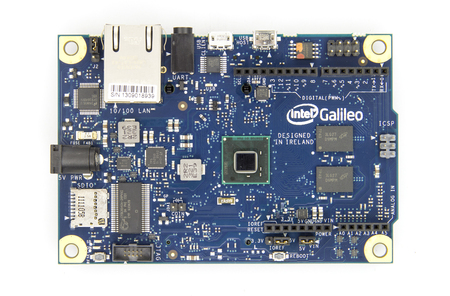
\includegraphics[width=8cm]{photos/galileo.jpg}
  \end{center}
\end{frame}

\begin{frame}
\frametitle{Galileo}

Intel verschenkt an Unis Galileo-Boards im Arduino-Shield-Layout. Das besondere: Statt Microcontroller kommt ein Pentium zum Einsatz:
\newline

\begin{itemize}
\item Intels Versuch, mit Embedded x86 in die N�he von Microcontrollern zu kommen
\item Referenzboard f�r Intels Quark SoC x1000
\item Arduino-Code wird in ELF-Objekte kompiliert
\item recht langsames IO
\item \emph{Mattias' Meinung:} The worst of both worlds
\end{itemize}
\end{frame}

\begin{frame}
\frametitle{Arduino Tre}
Gemeinsam mit TI und dem BeagleBone-Projekt entwickelter ,,janusk�pfiger'' Arduino aus TI Sitara und Atmega32u4, Leistung der Linux-Seite h�her als beim Raspberry Pi:

  \begin{center}
    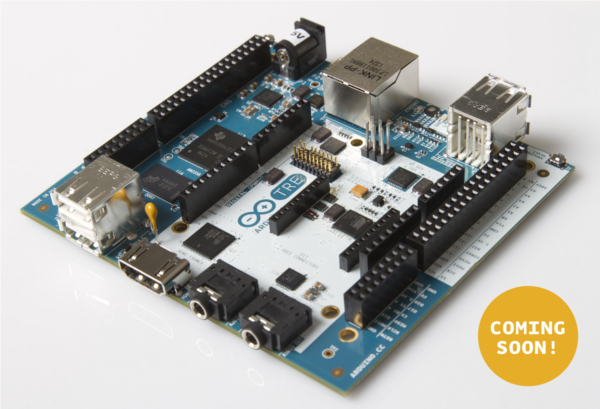
\includegraphics[width=8cm]{photos/arduinotre.jpg}
  \end{center}
\end{frame}

\begin{frame}
\frametitle{Arduino Tre}
Gemeinsam mit TI und dem BeagleBone-Projekt entwickelter ,,janusk�pfiger'' Arduino aus TI Sitara und Atmega32u4, Leistung der Linux-Seite h�her als beim Raspberry Pi:

\begin{itemize}
\item Von TI als Referenzplattform betrachtet
\item 100\% Code-Kompatibilit�t zu Arduino Leonardo
\item 100\% Code-Kompatibilit�t zu Beaglebone Black
\item recht teuer - Entwicklerkit 149 \euro - final 60 bis 80 \euro
\item \emph{Mattias' Meinung:} Tolles Konzept, hohe Leistung, aber hoher Preis und gro�e Platine
\end{itemize}
\end{frame}

\begin{frame}
\frametitle{Arduino Y�n}
Janusk�pfiger Arduino aus MIPS-Prozessor und Atmega32u4, Formfaktor des Uno, Leistung der Linux-Seite deutlich kleiner als beim Raspberry Pi, daf�r incl. WLAN und schnell angebundenem Ethernet:

  \begin{center}
    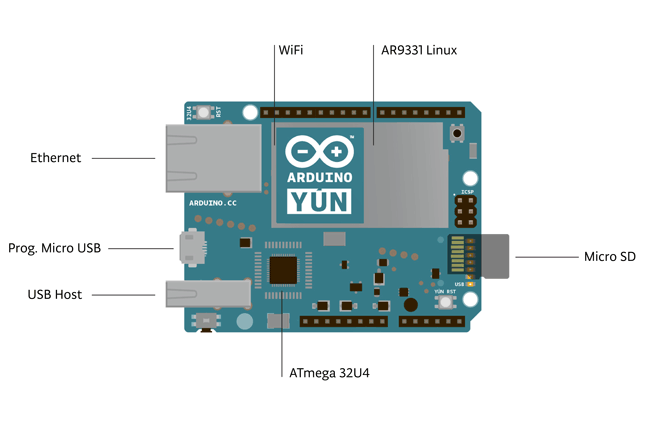
\includegraphics[width=8cm]{photos/YunParts.png}
  \end{center}
\end{frame}

\begin{frame}
\frametitle{Arduino Y�n}
Janusk�pfiger Arduino aus MIPS-Prozessor und Atmega32u4, Formfaktor des Uno, Leistung der Linux-Seite deutlich kleiner als beim Raspberry Pi, daf�r incl. WLAN und schnell angebundenem Ethernet:
\newline

\begin{itemize}
\item Eigenentwicklung mit Fokus auf guter Nutzbarkeit
\item 100\% Code-Kompatibilit�t zu Arduino Leonardo
\item OpenWRT basierte Distribution f�r die MIPS-Seite
\item Stra�enpreis 60 bis 75 \euro - kann parallel als WLAN Access Point genutzt werden
\item \emph{Mattias' Meinung:} Tolles Konzept, passende Leistung, sollte etwas g�nstiger sein
\item \emph{Der Clou:} Die Software - einfacher geht es nicht!
\end{itemize}
\end{frame}

\begin{frame}
\frametitle{Arduino Y�n - Software-Integration}
Eine neue Sammlung von Bibliotheken f�r die Arduino-IDE abstrahiert die Kommunikation zwischen Microcontroller- und Microprozessorseite:
\newline

\begin{itemize}
\item Bridge-Bibliothek f�r Zugriff auf viele Netzwerkfunktionen aus Arduino-Sketches - nur eine Programmiersprache n�tig!
\item ,,Mailbox'' (toter Briefkasten) f�r den Datenaustausch zwischen Microcontroller und Microprocessor
\item Integration von Temboo - abstrahiert verschiedene Webdienste
\item Voller Paketumfang von OpenWRT
\item Einfaches Webinterface f�r die Einrichtung - Luci bekannt von OpenWRT
\end{itemize}
\end{frame}

\begin{frame}
\frametitle{Arduino Y�n - Twitter-Beispiel}
  \begin{center}
    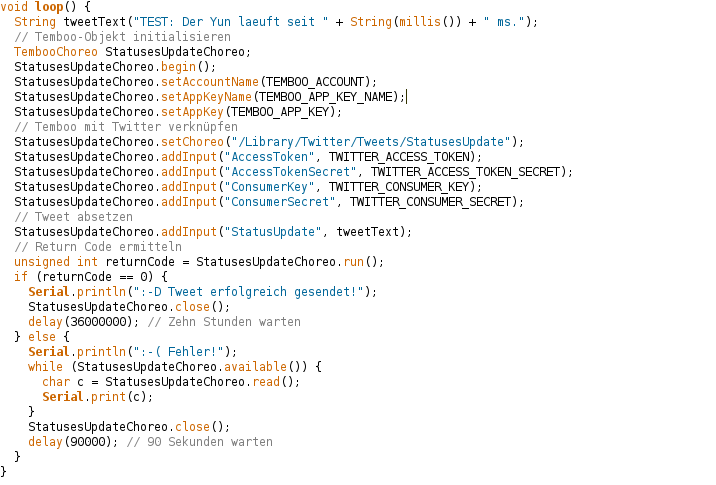
\includegraphics[width=10cm]{photos/codetwitter.png}
  \end{center}
\end{frame}


\subsection{Neue Microcontroller mit ARM-Kern}

